\section{Task 0: Validation of the Reference Design} \label{sec:task0}

Before modifying any RTL, the provided pixel-inversion example was run unchanged to confirm that the toolchain (Bender, the RISC-V cross-compiler and Questa) was complete and to obtain a known-good reference for the later Sobel design. In this design \texttt{pixel\_acc.sv} replaces every 8-bit pixel $p$ with $255-p$. All steps of the lab guide were executed on Windows~11 through \texttt{Makefile.win}.

\subsection{Dependencies and Firmware}

\texttt{make repository\_init} fetched all hardware dependencies (Ibex core, AXI/APB infrastructure, UART and SPI IPs) into \texttt{.bender/} and \texttt{vendor\_ips/} without errors. \texttt{make build\_test TEST=pixel\_inversion} then cross-compiled the reference firmware for the RV32IMC Ibex core, producing the \texttt{.elf}, the disassembly and the \texttt{.hex} file used to preload the instruction memory. The program occupies only 680 bytes, well within the available IMEM.

\subsection{Standalone Accelerator Simulation}

\texttt{make test\_ss} runs \texttt{tb\_student\_ss.sv}, which acts as an APB master towards \\ \texttt{Student\_area\_0}: it writes the 352$\times$288 image \texttt{pattern.pgm} into the input buffer (four pixels per 32-bit word), sets \texttt{DATA\_READY}, polls \texttt{DONE} and reads the output buffer back into \texttt{pattern\_result.pgm}. The CPU is not involved.

The simulation compiled without errors and reached \texttt{\$finish} with 0 errors. Since the testbench performs no automatic check, the output was compared pixel by pixel with the input: all 101\,376 pixels satisfy $p_{out} = 255 - p_{in}$. Figure~\ref{fig:task0_images} shows the expected photographic negative.

\begin{figure}[H]
    \centering
    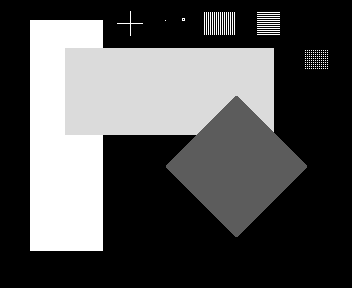
\includegraphics[width=0.45\textwidth]{figures/task0_pattern_in.png}\hfill
    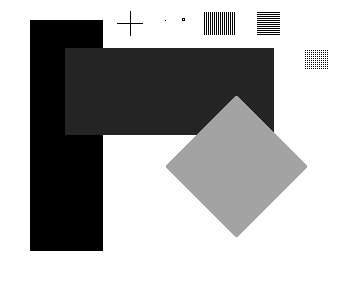
\includegraphics[width=0.45\textwidth]{figures/task0_pattern_inverted.png}
    \caption{Input image \texttt{pattern.pgm} (left) and output of the accelerator (right).}
    \label{fig:task0_images}
\end{figure}

Table~\ref{tab:task0_timing} breaks down the simulated time, running at 100\,MHz clock. The accelerator processes one word per cycle, 25\,344 cycles plus two for FSM start and pipeline drain, and takes only about 12.5\,\% of the run. The rest is APB transport. This gives a reference for the Sobel design: with a single 32-bit read port, about 25\,000 cycles is a practical lower bound on processing time.

\begin{table}[H]
\centering
\caption{Breakdown of the standalone simulation of the reference design.}
\label{tab:task0_timing}
\begin{tabular}{@{}lrr@{}}
\toprule
Phase & Cycles & Cycles/word \\
\midrule
Load input buffer over APB & $\approx$ 76\,000 & 3 \\
Accelerator (\texttt{start} $\rightarrow$ \texttt{finish}) & 25\,346 & $\approx$ 1 \\
Read output buffer over APB & $\approx$ 101\,400 & 4 \\
\bottomrule
\end{tabular}
\end{table}

\subsection{Waveform Inspection}

\texttt{make test\_ss\_gui} opened the same run in the Questa GUI with the preconfigured \texttt{wave\_ss.do}. The waveforms were used to understand the accelerator interface that the Sobel design must respect.

Figure~\ref{fig:task0_wave_start} shows the start of processing: the CPU-side write of \texttt{DATA\_READY} produces a one-cycle \texttt{acc\_start} pulse, after which the FSM enters \texttt{PROCESS} and increments \texttt{ibuf\_rd\_addr} every cycle. Because of the one-cycle BRAM read latency and the registered write port, the first output word is written two cycles after the first read.

\begin{figure}[H]
    \centering
    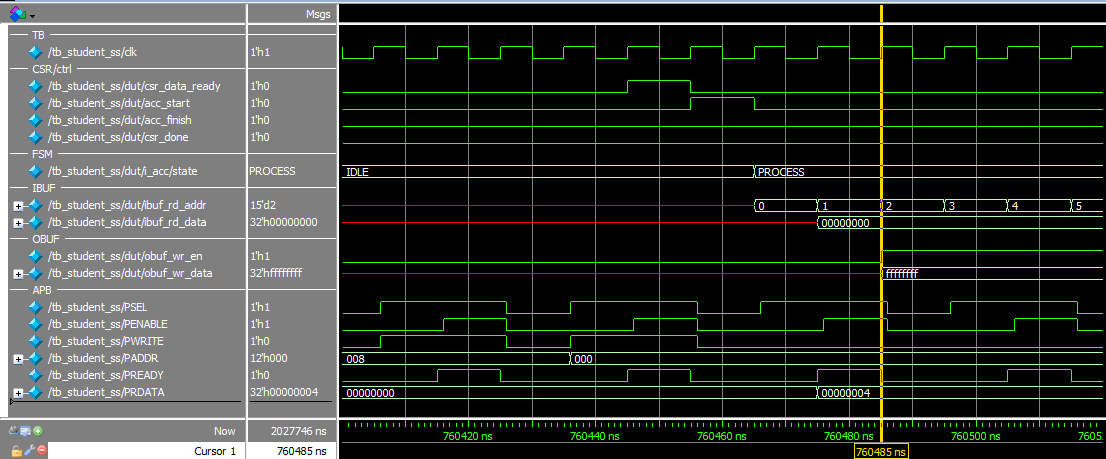
\includegraphics[width=\textwidth]{figures/task0_wave_start.png}
    \caption{Start of processing: \texttt{DATA\_READY}, the \texttt{acc\_start} pulse and the read/write pipeline of \texttt{pixel\_acc}.}
    \label{fig:task0_wave_start}
\end{figure}

Figure~\ref{fig:task0_wave_end} shows the end of the frame: after the last read the FSM spends one cycle in \texttt{DRAIN}, the last word is written together with the \texttt{acc\_finish} pulse, and \texttt{csr\_done} rises one cycle later. The testbench then reads the output buffer, where each APB read takes an extra wait state to cover the BRAM latency.

\begin{figure}[H]
    \centering
    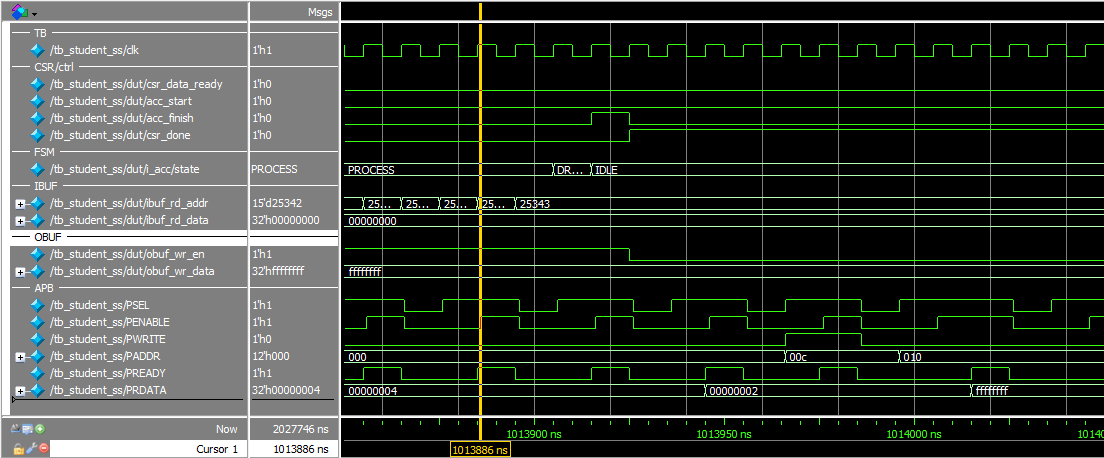
\includegraphics[width=\textwidth]{figures/task0_wave_end.png}
    \caption{End of processing: the \texttt{DRAIN} cycle, the last write with \texttt{acc\_finish}, the rise of \texttt{csr\_done} and the start of the APB read-back.}
    \label{fig:task0_wave_end}
\end{figure}

\subsection{Summary}

All four steps of Task~0 completed successfully: the dependencies were fetched, the firmware was built, and the standalone simulation produced a pixel-exact inverted image. The toolchain was therefore confirmed to work, and the \texttt{start}/\texttt{finish} handshake and BRAM timing observed here were kept unchanged for the Sobel accelerator described in the next section.
